The first thing you probably think of when you hear the word graph is plugging $y=mx+b$ into your calculator.  For the rest of this book, we'll refer to that concept as a plot.

A graph in a purely mathematical sense is a collection of {\bf nodes} and
{\bf branches}. Nodes are like locations or specific points in space, and
branches are the connections between the nodes (similar to pathways between the various locations).  You can draw a graph of this type as shown in Figure \ref{fig:graphTheory}.

% Figure of Example Graph
\begin{figure}
%  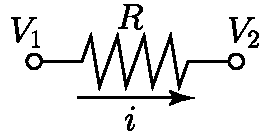
\includegraphics[width=0.5\linewidth]{figures/ohmsLaw}
  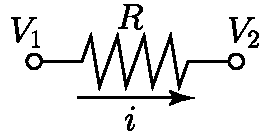
\includegraphics{figures/ohmsLaw}
  \caption{Pictured is a graph, which consists of a number of nodes and branches connecting those nodes.}
  \label{fig:graphTheory}
\end{figure}

We will be using the concept of a graph to talk about electric circuits.
